\documentclass[a4paper,12pt]{report}
    \title{Service Registry}
\author{Theodor Bogdan Vr\^ancean}
\date {Iunie 2018}

\usepackage[romanian]{babel}

\usepackage{graphicx}
\graphicspath{{"./Images/"}}

\usepackage[
    backend=biber,
    style=verbose,
    sorting=ynt
]{biblatex}
\addbibresource{References.bib}

\begin{document}
\maketitle
\tableofcontents
\chapter{Introducere}
\section{Arhitectura de microservicii}

Arhitectura de microservicii este o abrodare relativ nou\u a \^ in dezvoltarea de software.
Microserviciile reprezint\u a aplica\c tii mici \c si autonome care lucreaz\u a \^ impreun\u a
\footcite{buildingMicroservices}. Ele sunt considerate mici relativ la un sistem monolitic care ar
oferi toate func\c tionalit\u a\c tiile de care aplica\c tia are nevoie.Cu toate acestea un mictoserviciu poate oferi orice
fel de func\c tionalit\u a\c ti,incep\^and cu ceva simplu precum desc\u arcarea de fi\c siere, p\^an\u a la
complexe precum analizarea imaginilor.
Aceast\u a aboradare arhitecturala a venit ca o alternativ\u a la arhitectura monolitic\u a, \^in care exist\u a
un singur server care satisface toate necesit\u a\c tile unei aplica\c tii.Limit\u arile acestei abord\u ari ies la iveal\u a
odat\u a cu cre\c sterea aplica\c tiei.
Pentru a \^intelege de ce arhitectura  de microservicii \^incepe sa \^inlocuiasc\u a arhitectura monolitic\u a 
trebuie sa cunoa\c stem urm\u atoarele beneficii:
\begin{itemize}
	\item Din cauza dimensiunii \c si complexit\u a\c tii unui proiect monolitic,
	      acesta este dificil de in\c teles \c ,motiv pentru care schimb\u arile sunt mai dificil de facut \c si exist\u a
	      un risc mai mare ca acestea s\u a produc\u a efecte nedorite.Aceste probleme pot fi atenuate printr-un
	      cod de calitate dar acest lucru se \^ inatmpla de prea pu\c tine ori. Schimb\u arile aduse unui microserviciu nu afecteaz\u a alte
	      module \c si datorit\u a dimensiunii reduse a acestora, ele sunt \c si mai u\c sor de \^inteles pentru programtori, astfel
	      scade probabilitatea erorilor.Se poate spune ca microserviciile duc un pas mai departe principiul singurei responsabilit\u a\c ti,
	      definit de Robert C. Martin.
	\item Pentru dezvoltarea unei aplica\c tii monolitice trebuie sa alegem un tehnologii standardizate care s\u a poata
          realiza toate cerin\c tele aplica\c tiei. Pe de alta parte,daca avem mai multe microservicii care colaboreaz\u a nu exist\u a 
          aceast\u a limitare,ceea ne permite s\u a alegem unealta cea mai portivit\u a pentru fiecare serviciu.
          S\u a lu\u am spre exemplu un site al unei pizzerii care folose\c ste microservicii (Fig 1).
          Partea de front-end doar apeleaz\u a serviciile c\^and are nevoie.Putem avea un server scris 
          in C\# care folose\c ste un sistem de gestiune a bazei de date Microsoft Sql Server,
          unul scris \^in php cu MySql \c si unul scris in Node.js cu mongoDb \ref{fig:PizzaMicroservicii}.Deoarce toate comunic\u a prin
          protocolul http ,acestea pot lucra \^impreun\u a,fiecare av\^and responsabilitatea sa.
    \item O aplica\c tie a c\u arei componente sunt distribuite este mai rezistent\u a, \^in sensul c\u a dac\u a un 
          serviciu este compromis, func\c tionalita\c tile care nu depind de acel serviciu vor continua s\u a func\c tioneze.
          \^In cazul unei aplica\c tii clasice, tot sistemul va fi compromis din cauza unei singure componente.
          
          

\end{itemize}

\begin{figure}[!htb]
              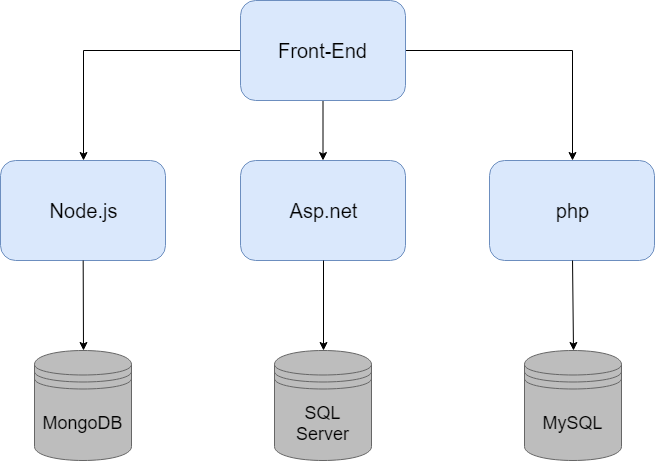
\includegraphics[width=\textwidth,keepaspectratio]{PizzaMicroservicii}
              \caption{Arhitectur\u a cu microservicii pentru un site de pizzerie}
              \label{fig:PizzaMicroservicii}
\end{figure}
Ele ofer\u a servicii care pot fi utilizate in de c\u atre alte aplica\c tii.
Printre avantajele aduse de microservicii, este faptul c\u a acestea pot fi utilizate de
mai multe aplica\c tii.\^In func\c tie de aceast\u a tr\u as\u atura microserviciile se pot impar\c ti \^in
trei categorii:





\chapter{Tehnologii}

C\# este un limbaj de programare. \^ s \c t \^a

\section{.Net Framework}
\section{Entity Framework}
EntityFramework este un ORM(Object Relational Mapper) open-source pentru platforma .Net.
\section{Asp.Net}
\section{MVC pattern}
\section{Microsoft Sql Server}

\chapter{Utilizare}

\end{document}
